\section{When MMIO Direct Push Collapses Itself}
\label{sec:device_collapse}

Even when a single host core stays well below the PCIe Gen5\,$\times$4 ceiling, naive MMIO direct push can collapse its \emph{own} throughput by 5$\times$--10$\times$---and, crucially, feed backpressure right back into the host \texttt{CHA TOR} cliff of \S\ref{sec:host_contention}. On our SPR--CN106 testbed, we isolate three tightly coupled device-side and ordering hazards: pre-\texttt{IIO} mesh reordering, Level-1 \texttt{Normal-WB} snoop serialization, and Level-2 \texttt{MT\_NORMAL\_NC} \texttt{EXLMN} frontier collisions.

\begin{figure*}[t]
  \centering
  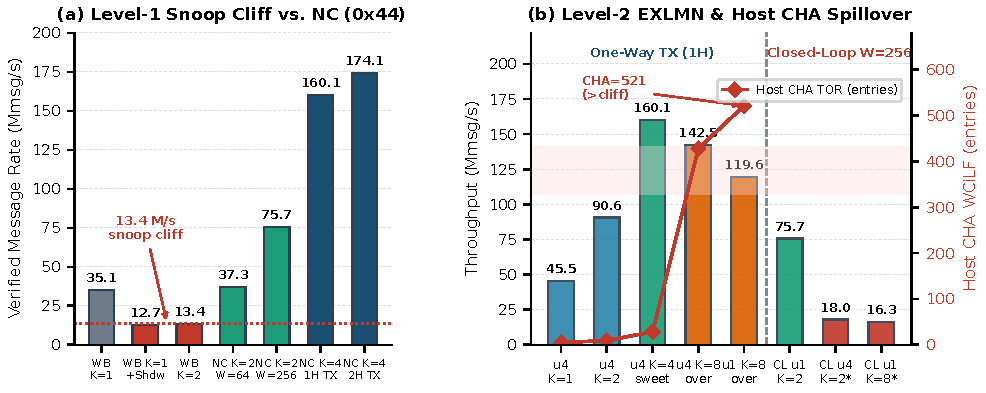
\includegraphics[width=\textwidth]{figures/fig2_device_self_collapse.pdf}
  \caption{Two-level device-side self-collapse and host spillover on CN106 \texttt{BAR4}. (a)~Level-1 collapse: under default \texttt{Normal-WB} pages, adding either a second active worker (\texttt{K=2}) or a single passive frontier-polling shadow core (\texttt{+Shdw}) drops throughput from 35.1 to 12.7--13.4\,Mmsg/s. Standard Linux \texttt{MT\_NORMAL\_NC} (\texttt{0x44}) eliminates private-cache snoops and scales to 160.1--174.1\,Mpps. (b)~Level-2 collapse: over-provisioning \texttt{MT\_NORMAL\_NC} (\texttt{K=8}) or tight multi-slot closed-loop polling (\texttt{CL u4 K=2}) triggers L3 \texttt{EXLMN} collisions (collapsing closed-loop to 16.3--18.0\,Mmsg/s) and overflows the device posted buffer back into host \texttt{CHA TOR} (428--521 entries, crossing the 330--430 cliff).}
  \label{fig:device_collapse}
\end{figure*}

\subsection{Pre-IIO Mesh Reordering and the Ordering Tax}
\label{sec:dev_order}

Posted PCIe \texttt{MWr} TLPs with \texttt{RO\,=\,0} are strictly ordered \emph{after} entering the root complex (\texttt{IIO1}), which tempts designers to omit host-side \texttt{SFENCE} when publishing multi-line messages or separate doorbells. Our measurements on CN106 \texttt{BAR4} show that this assumption fails \emph{before} \texttt{IIO1}, inside the host's 32-slice \texttt{CHA} mesh and multi-engine accelerators (\autoref{fig:ordering}a).

First, using sparse per-slot hardware timestamps across CN106 \texttt{BAR4} under un-fenced \texttt{MOVDIR64B}, 13.9\%--14.7\% of back-to-back writes issued within \texttt{$<$25\,ns} arrive out of program order at CN106 because consecutive 64\,B lines hash to \texttt{CHA} slices at different 2D-mesh hop distances from \texttt{IIO1} (dropping to 0.0\% once issue spacing exceeds 40\,ns). Second, in a dedicated 204-run multi-line ordering audit (6,000,000 verified writes, 0 persistent errors) where a CN106 core spins with \texttt{ldar} on the tail 64\,B line and immediately snapshots all preceding lines:
\begin{itemize}
  \item \textbf{Un-fenced CPU \texttt{MOVDIR64B}} exhibits 2.21\%--4.99\% transient reordering on 512\,B payloads and 3.79\%--5.89\% on 1\,KiB payloads (and shifting a 128\,B block to \texttt{BAR4+896} still reorders $\sim$4.2\%). Inserting a single \texttt{SFENCE} before the tail line drops reordering to 0 / 270,000 (0.00\%).
  \item \textbf{Multi-engine Intel DSA} pushing a 4\,KiB payload followed by a 64\,B doorbell to \texttt{BAR4} reorders 96.89\%--99.09\% of doorbells ahead of payload completion on 4 engines when submitted back-to-back (\texttt{FENCE\,=\,0}); inserting a standalone \texttt{DSA\_OPCODE\_DRAIN} still reorders 96.16\%--99.09\% because \texttt{DRAIN} does not prevent an idle engine from dispatching the subsequent doorbell. Only \texttt{Batch(2)} with \texttt{IDXD\_OP\_FLAG\_FENCE\,=\,1} (0 / 360,000, adding +299--426\,ns) or waiting for \texttt{dsa\_comp} on the host followed by \texttt{SFENCE + MOVDIR64B} (0 / 360,000 at \texttt{W\,=\,1}, saving $\sim$0.6--0.7\,\textmu s) achieves strict ordering.
\end{itemize}
For 64\,B single-line messages, \texttt{MOVDIR64B} is atomic within a line and needs no per-message \texttt{SFENCE} if the receiver detects arrival via per-slot generation stamps. For decoupled doorbells or multi-line messages, however, omitting \texttt{SFENCE} causes real silent races (2,356--11,539 doorbell-ahead-of-data inversions in un-fenced per-packet trials), while issuing \texttt{SFENCE} on every single 64\,B packet caps host throughput to $\sim$7--14\,Mmsg/s. Ordering must therefore be amortized across batches (\S\ref{sec:design}).

\subsection{Level-1 Self-Collapse: Normal-WB Snoop Cliff}
\label{sec:dev_wb}

On CN106, when host \texttt{cpu40} pushes 64\,B \texttt{MOVDIR64B} writes into \texttt{BAR4} without receiver polling, throughput reaches 162.1\,Mmsg/s (1 host core) and 175.2\,Mmsg/s (4 host cores). Yet when two or more ARM cores poll the default cacheable (\texttt{Normal-WB}, \texttt{0xFF}) ring buffer in closed loop (\texttt{W\,=\,64}, 128\,B slot stride to avoid false sharing), throughput collapses by more than an order of magnitude to 13.1--13.5\,Mmsg/s (\autoref{fig:device_collapse}a), and RTT jumps from 0.90\,\textmu s to 3.90--4.62\,\textmu s.

Three controlled microbenchmarks pinpoint the exact root cause:
\begin{enumerate}
  \item \textbf{Not a \texttt{TAD} total-snoop limit:} Pure on-chip \texttt{ARM\,$\leftrightarrow$\,ARM} ring transfers (zero PCIe) scale \texttt{TAD} snoop bandwidth linearly from 94.2 to 730.6\,M\,snoops/s across 1--8 core pairs without saturating---17.3$\times$ higher than the 42.2\,M\,snoops/s observed during the 13.4\,M/s \texttt{BAR4} stall.
  \item \textbf{Shared inbound-bridge serialization (\texttt{PEM0}/\texttt{IOBN}):} Splitting \texttt{BAR4} slot~15 into $K\,=\,1, 2, 4$ completely independent sub-rings spaced 960\,KiB apart (spanning all \texttt{TAD} slices) with dedicated host and card cores locks \emph{aggregate} throughput at 13.42 / 13.39 / 13.39\,Mmsg/s---dividing each independent ring to exactly $13.4 / K$\,Mmsg/s while both host \texttt{CHA} (1.38 entries) and card \texttt{TAD} (0.02 entries) sit nearly empty.
  \item \textbf{Causal trigger---active frontier polling under \texttt{Normal-WB}:} On a healthy 1-core closed-loop baseline running at 35.06\,Mmsg/s (where hardware L2 prefetching already causes 0.99 \texttt{L2D\_CACHE\_INVAL} (\texttt{0x58}) per message without serializing), adding a \emph{single} shadow core that neither consumes nor replies---merely spinning on the unwritten frontier slot \texttt{front+0} or \texttt{front+4}---immediately crashes throughput by $-$64\% to 12.70 / 12.50\,Mmsg/s (shadow-core \texttt{0x58} jumps from 0.05 to 1.30--1.41/msg; a control shadow core spinning on a private line leaves throughput at 35.33\,Mmsg/s).
\end{enumerate}

Crucially, \emph{no instruction-level fix on \texttt{Normal-WB} pages escapes this cliff}. Removing the shared \texttt{next\_offset} line (13.12\,M/s), relaxing \texttt{ldar} to \texttt{ldr}, \texttt{ldr+dmb}, or non-temporal \texttt{ldnp} (13.43--13.47\,M/s, 0.3\% spread), sleeping with \texttt{LDAXR+WFE} (12.41\,M/s, because \texttt{LDAXR} still installs the line in L1D), or explicitly evicting with \texttt{DC CIVAC} (11.50\,M/s, triggering 0.41/msg DDR5 writebacks) all remain trapped. Even classic software skipping---\texttt{B-Queue} adaptive probing~\cite{wang2013bqueue} (\texttt{next+D-1} + binary backtrack)---backfires catastrophically: failed probes prefetch unwritten slots into private L1D/L2, planting ``snoop mines'' that drop 1-core throughput from 34.24 down to 13.53\,Mmsg/s (\autoref{fig:ordering}b). Whenever an active receiver holds an unwritten frontier line in private L1/L2, the arriving PCIe posted write must stall in \texttt{PEM0}/\texttt{IOBN} behind a coherent snoop invalidation handshake (76.4\,ns per write = 13.1\,M/s), and PCIe posted ordering head-of-line-blocks every write behind it.

\begin{figure*}[t]
  \centering
  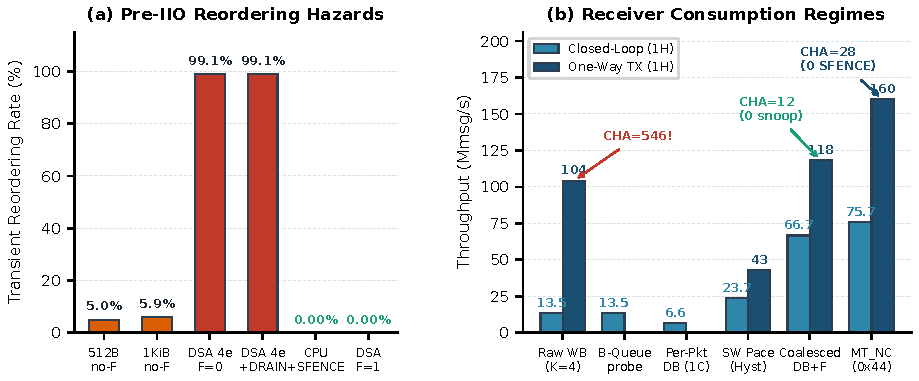
\includegraphics[width=\textwidth]{figures/fig3_ordering_and_doorbell.pdf}
  \caption{Ordering hazards and receiver-consumption trade-offs on CN106 \texttt{BAR4}. (a)~Transient out-of-order arrival rates: un-fenced \texttt{MOVDIR64B} (512\,B--1\,KiB) reorders 2.2\%--5.9\% across the 32-\texttt{CHA} mesh, and 4-engine DSA back-to-back writes reorder 96.2\%--99.1\% even with \texttt{DRAIN}; \texttt{SFENCE} and \texttt{DSA Batch FENCE=1} eliminate reordering (0.00\%). (b)~Head-to-head comparison of six receiver regimes (1 host core): raw \texttt{Normal-WB}, \texttt{B-Queue}, and per-packet doorbells collapse; coalesced doorbell+\texttt{SFENCE} sustains 66.7\,M/s closed-loop and 118.2\,M/s one-way at \texttt{CHA\,=\,12}; \texttt{MT\_NORMAL\_NC} reaches 75.8\,M/s closed-loop and 160.1\,M/s one-way with zero \texttt{SFENCE}.}
  \label{fig:ordering}
\end{figure*}

\subsection{Level-2 Self-Collapse: \texttt{MT\_NORMAL\_NC}, \texttt{EXLMN}, and Host Spillover}
\label{sec:dev_nc}

Because ring messages are read once by a card core and then overwritten by PCIe, caching them in private L1D/L2 offers no reuse while paying a 10$\times$ snoop penalty. Remapping the card's ring buffer with standard Linux \texttt{MT\_NORMAL\_NC} (\texttt{0x44})---requiring \emph{zero} modification to ARMv8 \texttt{MAIR\_EL1}---breaks the Level-1 cliff cleanly. On OCTEON~10 CN106, the 48\,MiB shared L3 (\texttt{TAD}) serves as the CHI Point of Coherence and satisfies \texttt{MT\_NORMAL\_NC} reads directly from L3 without touching DRAM: across 147 controlled runs, standard \texttt{0x44} matched a custom \texttt{Inner-NC, Outer-WB} (\texttt{0xF4}) \texttt{MAIR} attribute within $\pm$0.1\%, drove \texttt{l1d\_refill}, \texttt{0x58 L2D\_CACHE\_INVAL}, and \texttt{DDR5} reads all to 0.00, and cut total \texttt{TAD} snoops by $-$98\%. Paired with a single-pass \texttt{4$\times$ldp} load (which Neoverse N2 coalesces into one 64\,B \texttt{ReadOnce}), \texttt{MT\_NORMAL\_NC} preserves unloaded \texttt{W\,=\,1} RTT at 900.9--901.8\,ns (only +12\,ns over \texttt{WB ldar}) and scales in one-way TX to 160.10\,Mpps (1 host core, 99.0\% of link ceiling, \texttt{CHA\,=\,28.2}) and 174.10\,Mpps (2 host cores, 99.4\% of ceiling) using just $K\,=\,4$ card cores with 4-slot unrolling (\texttt{u4}) and zero \texttt{SFENCE} (\autoref{fig:device_collapse}a).

\para{Why \texttt{MT\_NORMAL\_NC} alone is not enough.}
Bypassing private L1D/L2 removes the \texttt{Normal-WB} snoop tax, but introduces a second-order trade-off: every empty poll now misses private cache and penetrates straight to the shared \texttt{TAD} L3. When card cores stay slightly behind the incoming write stream, empty polls are negligible and \texttt{MT\_NORMAL\_NC} flies. When card cores outpace the producer and hammer the unwritten write frontier, however, non-cacheable \texttt{TAD} reads collide directly with arriving PCIe writes at the same 128\,B \texttt{TAD} line, triggering CHI exclusive-line-monitor/coherence retries (\texttt{tad\_snp\_msh\_out\_exlmn} jumps from 0.02/msg at \texttt{u4 K=4} to \texttt{$>$1.06}/msg!):
\begin{itemize}
  \item \textbf{Closed-loop \texttt{EXLMN} collapse (\autoref{fig:device_collapse}b):} Running the exact same \texttt{u4} tight-polling loop that achieved 160.1\,Mpps one-way in a closed-loop \texttt{W\,=\,256} workload collapses throughput by 4.2$\times$ to 17.96\,Mmsg/s (\texttt{p99\,=\,15.2\,\textmu s}). Even conservative \texttt{u1} polling collapses to 16.27\,Mmsg/s (\texttt{H\,=\,1, K\,=\,8, W\,=\,256}) and 22.84\,Mmsg/s (\texttt{H\,=\,2, K\,=\,8, W\,=\,512}) once card cores are over-provisioned.
  \item \textbf{Posted-buffer overflow back into host \texttt{CHA TOR}:} Under wide-window one-way TX (\texttt{W\,=\,6144}, \texttt{H\,=\,1}), over-provisioning card cores from $K\,=\,4$ to $K\,=\,8$ not only degrades throughput (160.1\,$\to$\,142.5\,Mpps for \texttt{u4}; 136.8\,$\to$\,119.6\,Mpps for \texttt{u1}), it slows card-side drain enough to fill CN106's $\sim$387--391-slot inbound posted buffer and push backpressure \emph{upstream across PCIe into the host}: socket-wide host \texttt{CHA WCiLF} surges from a harmless 14.4--28.2 entries straight to 428.1 (\texttt{u4 K=8}) and 521.2 (\texttt{u1 K=8}; 546.2 on raw \texttt{WB K=4})---squarely inside the 330--430 neighbor-collapse cliff of \S\ref{sec:host_contention}!
\end{itemize}
This closes the causal loop: unpaced host injection and unpaced device polling are not isolated phenomena; either one can overflow the finite posted pipeline and starve the entire host socket.
